\subsection{Purpose}
\label{intro:purpose}
This document specifies the Software Requirements Specification for the \textit{TaskManager For Tomboy} project.
It describes scope of the system, both functional and non-functional requirements for the software, system interfaces and existing previous solutions.


\subsection{Scope}
\label{intro:scope}
The project TaskManager is an Addin for Tomboy that will enhance Tomboy with the possibility to do task management. 
The user will be able to create and manage task notes, i.e. adding and removing tasks to task lists and link other task notes in some tasks.
Simple task entries will be enhancable with optional arguments such as due dates and priority.
The user will be able to use Tomboy intuitively as a task management system for daily usage, without prior explanation or documentation. 
The Addin will integrate nicely within the existing concepts and GUI elements of Tomboy.

This is how the final result could look like. Figure \ref{gui} is only a draft, trying to visualize how the integration into Tomboy can be accomplished. You can see a checkbox before each task to mark this particular task as done, along with the corresponding priorities on the left side and due dates on the right side.
\begin{figure}[h]
  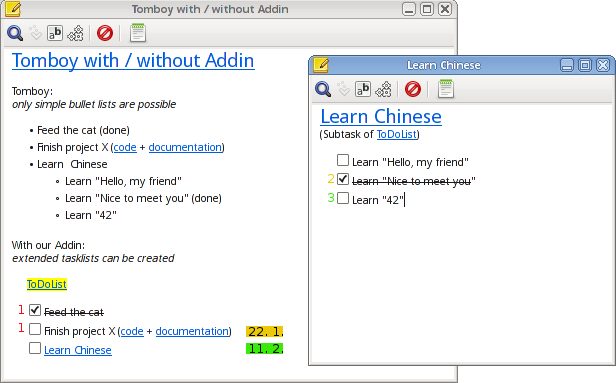
\includegraphics[width=\textwidth]{graphics/Screenshot_cropped_edited.png}
  \caption{GUI mockup}
  \label{gui}
  \index{GUI}
\end{figure}


\subsection{Acronyms and abbreviations}
\label{intro:abbreviations}
The following table explains the terms and abbreviations used in the document.
\\*
\\*
\begin{objects}
	% Make sure to maintain alphabetical order
	\object{CLI}{Common Language Infrastructure}
	\object{C\#}{C-Sharp}
	\object{GTK}{GIMP ToolKit}
	\object{GTK\#}{Gtk Sharp}
	\object{GUI}{Graphical User Interface \index{GUI}}
	\object{XML}{Extensible Markup Language}
\end{objects}


\subsection{Definitions}
\label{intro:definitions}
These definitions are terms we use to describe specific concepts within our product.
\\*
\\*
\begin{objects}
	% Make sure to maintain alphabetical order
	\object{Task}{A task is a piece of text representing a ``todo'' item, accompanied with a checkbox.

It may have a due date, a priority and can be marked as done. \index{Task}}
	\object{Task List}{A task list is a collection of tasks that is grouped together.

It may have a title, a priority and a due date. \index{Task List}}
        \object{Task Note}{A task note is a Tomboy Note enhanced with the TaskManager features. \index{Task Note}}
	\object{Subtask}{A subtask is a task note being linked from inside a task. \index{Subtask}}
\end{objects}


\subsection{Glossary}
\label{intro:glossary}
The glossary defines the key terms and concepts mentioned and used in this SRS.
\\*
\\*
\begin{objects}
	% Make sure to maintain alphabetical order
	\object{Addin}{An extension for a particular Product that can be enabled and disabled, as needed.} %TODO capitalized or not in text?
        \object{CLI Standard}{TODO} %TODO
	\object{Cross Platform}{Attribute conferred to computer software which is implemented and inter-operates on multiple computer platforms.}
	\object{C-Sharp}{Programming Language for the CLI Standard.}
	\object{Evolution}{The official personal information manager and workgroup information management tool for GNOME. }
	\object{GIMP ToolKit}{A cross platform widget library for creating GUIs.}
	\object{GNOME}{A desktop environment (a graphical user interface that runs on top of a computer operating system) composed entirely of free and open source software.}
	\object{GTK Sharp}{GTK Language Bindings for C\#}
	\object{Mono}{Cross Platform .NET Compatible Open Source implementation of the CLI Standard.}	
	\object{Tomboy}{A free and open-source desktop notetaking application written for Unix-like (including Mac OS X) and Microsoft Windows systems. Tomboy is part of GNOME and written in C\# using Gtk\#. \index{Tomboy}}
	\object{User}{Any Person who uses Tomboy.}
	\object{Widget}{An element of a GUI that displays an information arrangement changeable by the user.}
	\object{.NET Framework}{Microsofts Implementation of the CLI Standard.}
\end{objects}


\subsection{References}
\label{intro:references}
The following table defines the list of all documents referenced elsewhere in these requirements.
\\*
\\*
\begin{reference_table}
  \reference{Tomboy Styleguide}{\label{styleguide} \url{http://projects.gnome.org/tomboy/TODO} }
  \reference{LGPL}{\label{lgpl} \index{LGPL} \url{http://www.gnu.org/licenses/lgpl.txt}}
  \reference{IEEE 830-1998}{\label{ieee} \url{http://standards.ieee.org/reading/ieee/std/se/830-1998.pdf}}
  \reference{ICAL Specification}{\label{ical} \index{ICAL} \url{http://tools.ietf.org/html/rfc5545}}
  \reference{CLI Standard}{\label{cli} \index{cli} \url{TODO}}%TODO
\end{reference_table}


\subsection{Overview}
\label{intro:overview}
\begin{itemize}
  \item Chapter \ref{description} defines the general product functions, intended application, constraints to be respected and the assumption made in order to define requirements.
  \item Chapter \ref{requirements} specifies functional (section \ref{requirements:functional}) and non-functional requirements (usability, reliability, performance, maintainability, etc., sections \ref{requirements:nonfunctional_start} to \ref{requirements:nonfunctional_end}).

The level of detail there should be sufficient to enable designers to design a system satisfying these requirements and testers to test that the system satisfies these requirements.
  \item Chapter \ref{appendix} contains the appendix, which includes the index.
\end{itemize}
The document is structured according to the IEEE 830-1998 standard (see \ref{ieee}).
